\section{Expérimentations et résultats}

\subsection{Environnement de simulation}
Windows~11 Pro, processeur Intel à 12 threads logiques, Python~3.13.2 (versions des bibliothèques au §\ref{sec:impl}). Aucun GPU n'est utilisé : tous les modèles (y compris l'ANN, un \texttt{MLPClassifier}) s'exécutent sur CPU. Les temps sont des durées réelles mesurées avec \texttt{n\_jobs=-1} (12 processus). Sauf mention contraire, les résultats portent sur le \textbf{jeu de test} (30\,\%, 787 lignes dans le régime complet, 69 dans le régime propre).

\subsection{Résultats du baseline}
\begin{table*}[t]\centering\caption{Baseline (hyperparamètres par défaut), régime complet, \emph{toutes variables}, jeu de test. F1$_p$ : $F_1$ pondéré ; F1$_m$ : $F_1$ macro. En gras : meilleure valeur de la colonne.}\label{tab:baseline}
\footnotesize\begin{tabular}{lcccccccccc}
\toprule
& \multicolumn{5}{c}{Binaire} & \multicolumn{5}{c}{4 classes} \\ \cmidrule(lr){2-6}\cmidrule(lr){7-11}
Modèle & Acc. & F1$_p$ & F1$_m$ & AUC & AUC-PR & Acc. & F1$_p$ & F1$_m$ & AUC & AUC-PR \\
\midrule
LR & 0,756 & 0,737 & 0,661 & 0,742 & 0,594 & 0,757 & 0,725 & 0,501 & 0,745 & 0,535 \\
RF & \textbf{0,878} & \textbf{0,875} & \textbf{0,844} & \textbf{0,928} & \textbf{0,876} & \textbf{0,872} & \textbf{0,866} & \textbf{0,706} & \textbf{0,895} & \textbf{0,733} \\
KNN & 0,811 & 0,807 & 0,761 & 0,830 & 0,657 & 0,795 & 0,786 & 0,577 & 0,808 & 0,513 \\
SVM & 0,807 & 0,798 & 0,744 & 0,822 & 0,698 & 0,802 & 0,789 & 0,588 & 0,810 & 0,566 \\
NB & 0,708 & 0,706 & 0,639 & 0,712 & 0,495 & 0,682 & 0,676 & 0,384 & 0,740 & 0,455 \\
ANN & 0,841 & 0,839 & 0,801 & 0,853 & 0,764 & 0,821 & 0,815 & 0,627 & 0,847 & 0,592 \\
\bottomrule
\end{tabular}
\end{table*}

Le tableau~\ref{tab:baseline} reproduit les tableaux~5 et~9 de \cite{bader2024}. Le \textbf{classement qualitatif est celui de l'article} : la RF est la meilleure sur toutes les métriques (AUC 0,928 en binaire, 0,895 à quatre classes), devant l'ANN (0,853 / 0,847), tandis que LR et NB sont les plus faibles (AUC de 0,71 à 0,75). En valeur absolue, nos AUC sont toutefois nettement supérieures à celles de l'article (0,84 et 0,88 pour la RF), ce qui n'est pas attendu avec moins de biomarqueurs.

Le cas des biomarqueurs seuls est révélateur (annexe~\ref{app:full}) : la RF y atteint une AUC de \textbf{0,936} (binaire), \emph{supérieure} à celle obtenue avec toutes les variables (0,928), alors que l'article observe l'inverse (0,81 puis 0,84). Dans le même temps, LR et NB restent au niveau du hasard (0,54 et 0,50), conformément aux corrélations quasi nulles : seul un modèle capable de \og mémoriser \fg{} des combinaisons exactes de valeurs réussit, ce qui est cohérent avec l'audit de la section~4.1. Les matrices de confusion (figure~\ref{fig:cm}) montrent que la classe sévère est correctement reconnue dans 5 cas sur 9 et la classe modérée dans 8 sur 22 pour la RF par défaut.

\begin{figure}[t]\centering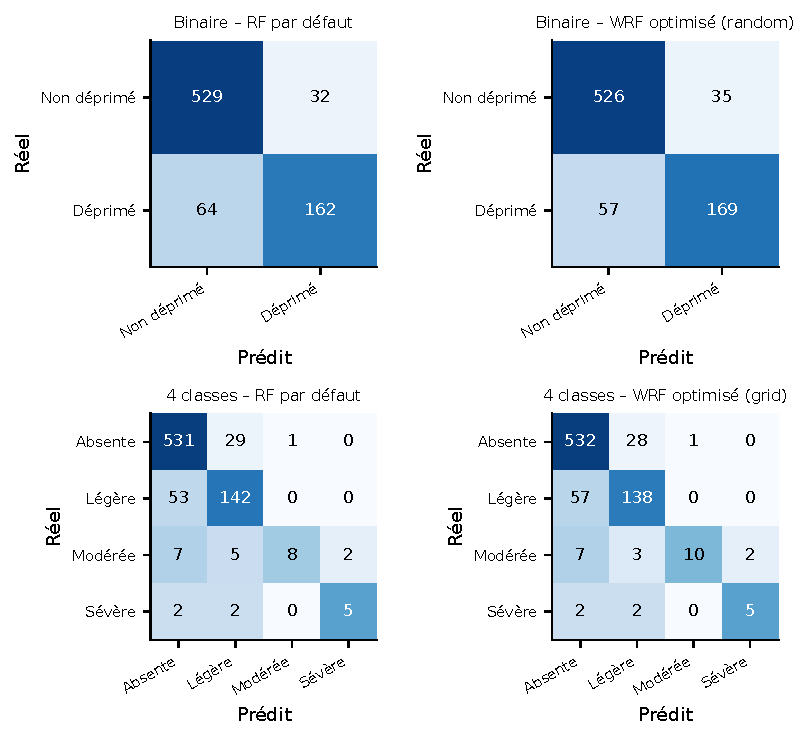
\includegraphics[width=\columnwidth]{../figures/confusion_matrices.pdf}
\caption{Matrices de confusion sur le test (toutes variables, régime complet) : RF par défaut et WRF optimisée, binaire (haut) et quatre classes (bas).}\label{fig:cm}\end{figure}

\subsection{Résultats des améliorations}
\paragraph{(A) Optimisation d'hyperparamètres.} Le tableau~\ref{tab:ba} compare les AUC avant et après optimisation. Dans le \textbf{régime complet}, les ensembles d'arbres sont déjà à leur plafond : la RF passe de 0,928 à 0,926 en binaire, alors que son AUC en validation croisée progresse de 0,935 à 0,942 (tableau~\ref{tab:time}) : le gain observé \emph{en validation} ne se retrouve pas \emph{sur le test}. Les modèles plus sensibles aux réglages gagnent davantage : KNN $+0{,}05$ (binaire) et $+0{,}09$ (quatre classes), SVM $+0{,}02$ à $+0{,}04$. Avec les biomarqueurs seuls, SVM et ANN gagnent jusqu'à $+0{,}14$ et $+0{,}08$ (annexe~\ref{app:full}). Pour la WRF à quatre classes, l'optimisation fait passer l'AUC de 0,903 à 0,927 (grille), 0,919 (aléatoire) et 0,915 (Optuna), valeur proche des 0,91 de l'article, mais les intervalles de confiance se chevauchent largement (tableau~\ref{tab:boot}). Dans le \textbf{régime propre}, l'optimisation n'améliore pas la RF (0,695 $\to$ 0,644 pour la grille) et les écarts restent dans l'incertitude ($\pm 0{,}14$).

\begin{table*}[t]\centering\caption{AUC sur le test avant (Déf.) et après optimisation (Grid, Rand.), toutes variables. En gras : meilleure valeur lorsqu'elle améliore le réglage par défaut.}\label{tab:ba}
\footnotesize\begin{tabular}{lccccccccc}
\toprule
& \multicolumn{3}{c}{Complet, binaire} & \multicolumn{3}{c}{Complet, 4 classes} & \multicolumn{3}{c}{Propre, binaire} \\\cmidrule(lr){2-4}\cmidrule(lr){5-7}\cmidrule(lr){8-10}
Modèle & Déf. & Grid & Rand. & Déf. & Grid & Rand. & Déf. & Grid & Rand. \\
\midrule
LR & 0,742 & 0,742 & \textbf{0,742} & 0,745 & \textbf{0,760} & 0,755 & 0,664 & 0,664 & \textbf{0,673} \\
RF & 0,928 & 0,926 & 0,926 & 0,895 & 0,895 & \textbf{0,906} & 0,695 & 0,644 & 0,682 \\
KNN & 0,830 & 0,877 & \textbf{0,880} & 0,808 & \textbf{0,895} & 0,894 & 0,724 & 0,682 & \textbf{0,726} \\
SVM & 0,822 & \textbf{0,837} & 0,824 & 0,810 & \textbf{0,851} & 0,836 & 0,642 & 0,645 & \textbf{0,646} \\
NB & 0,712 & \textbf{0,713} & 0,712 & 0,740 & \textbf{0,743} & 0,742 & 0,634 & 0,634 & 0,634 \\
ANN & 0,853 & 0,854 & \textbf{0,861} & 0,847 & \textbf{0,854} & 0,851 & 0,627 & \textbf{0,654} & 0,645 \\
\midrule
WLR & 0,739 & \textbf{0,739} & 0,739 & 0,688 & 0,669 & \textbf{0,703} & 0,661 & 0,663 & \textbf{0,665} \\
WRF & 0,923 & \textbf{0,928} & 0,925 & 0,903 & \textbf{0,927} & 0,919 & 0,665 & 0,668 & \textbf{0,705} \\
RF-SMOTE & 0,924 & 0,924 & 0,919 & 0,897 & \textbf{0,911} & 0,891 & 0,727 & 0,706 & 0,724 \\
WHGB & 0,915 & 0,920 & \textbf{0,927} & 0,910 & \textbf{0,916} & 0,915 & 0,683 & \textbf{0,700} & 0,683 \\
\bottomrule
\end{tabular}
\end{table*}

Les hyperparamètres retenus changent de nature selon le régime (figure~\ref{fig:hp}). Dans le régime complet, l'AUC en validation croisée augmente de façon monotone avec la profondeur et diminue quand \texttt{min\_samples\_leaf} croît : l'optimum est l'arbre entièrement développé (\texttt{max\_depth=None}, \texttt{min\_samples\_leaf=1}), avec KNN à pondération par la distance et un SVM à forte capacité ($C\approx 46$, $\gamma\approx 0{,}1$). Dans le régime propre, la surface est quasi plate (0,66--0,72) et favorise des arbres peu profonds (profondeur 3, feuilles de 3) et un SVM très régularisé ($C\approx 0{,}04$) : la recherche y exploite surtout le bruit de la validation croisée.

\begin{figure*}[t]\centering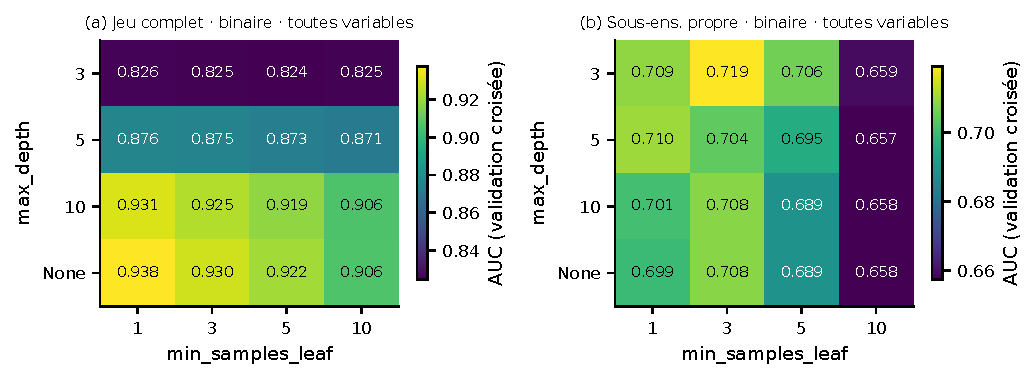
\includegraphics[width=0.78\textwidth]{../figures/hp_sensitivity.pdf}
\caption{Sensibilité de la RF à \texttt{max\_depth} et \texttt{min\_samples\_leaf} (AUC en validation croisée, grille moyennée sur \texttt{n\_estimators} et \texttt{max\_features}).}\label{fig:hp}\end{figure*}

\paragraph{(B) Pondération, SMOTE et modèle ajouté.} Le tableau~\ref{tab:weighted} confirme l'ordre de l'article à quatre classes (WRF $>$ RF-SMOTE $>$ WLR) : AUC de 0,903, 0,897 et 0,688 par défaut. La WLR s'effondre (exactitude 0,48, $F_{1,m}$ 0,33) : avec des poids atteignant $W\approx 21$ pour la classe sévère, un modèle linéaire sur-prédit les classes rares. La WRF améliore peu l'exactitude équilibrée de la RF (0,644 par défaut, 0,667 optimisée, contre 0,648) ; en binaire elle n'apporte rien (0,923 contre 0,928). Le modèle ajouté, WHGB, est compétitif : meilleur $F_{1,m}$ (0,738) et meilleure exactitude équilibrée (0,693) à quatre classes par défaut.

\begin{table}[t]\centering\caption{Modèles pondérés avant/après optimisation (méthode retenue d'après l'AUC en validation croisée), régime complet, \emph{quatre classes}, toutes variables ; Acc.$_{éq}$ : exactitude équilibrée.}\label{tab:weighted}
\scriptsize\begin{tabular}{lcccccc}
\toprule
\multicolumn{7}{l}{\textit{Complet, 4 classes, toutes var.}} \\ \midrule
Modèle & Acc. & F1$_p$ & F1$_m$ & Acc.$_{éq}$ & AUC & AUC-PR \\
\midrule
RF & 0,872 & 0,866 & 0,706 & 0,648 & 0,895 & 0,733 \\
RF (grid) & 0,869 & 0,865 & 0,726 & 0,669 & 0,895 & 0,743 \\
WLR & 0,478 & 0,562 & 0,329 & 0,490 & 0,688 & 0,371 \\
WLR (random) & 0,546 & 0,612 & 0,327 & 0,467 & 0,703 & 0,487 \\
WRF & 0,869 & 0,863 & 0,717 & 0,644 & 0,903 & 0,746 \\
WRF (grid) & 0,870 & 0,865 & 0,726 & 0,667 & 0,927 & 0,748 \\
RF-SMOTE & 0,844 & 0,843 & 0,685 & 0,661 & 0,897 & 0,723 \\
RF-SMOTE (grid) & 0,849 & 0,848 & 0,694 & 0,665 & 0,911 & 0,711 \\
WHGB & 0,875 & 0,874 & 0,738 & 0,693 & 0,910 & 0,756 \\
WHGB (random) & 0,874 & 0,873 & 0,720 & 0,690 & 0,915 & 0,725 \\
WRF (optuna) & 0,861 & 0,857 & 0,736 & 0,665 & 0,915 & 0,740 \\
\bottomrule
\end{tabular}
\end{table}

\paragraph{Courbes ROC et d'apprentissage.} Les courbes ROC des RF, WRF et RF-SMOTE se superposent presque dans le régime complet (figure~\ref{fig:roc}a), alors qu'elles sont très irrégulières et mêlées dans le régime propre (figure~\ref{fig:roc}b), où le test ne compte que 19 cas positifs. À quatre classes, la classe modérée est la moins bien séparée (figure~\ref{fig:roc}c). Les courbes d'apprentissage (figure~\ref{fig:lc}) montrent une AUC d'entraînement égale à 1 dans le régime complet et une AUC de validation qui progresse encore à pleine taille (0,92 à 0,94) : l'ajout de données serait plus utile que l'optimisation. Dans le régime propre, la validation plafonne vers 0,66 avec un écart-type large.

\begin{figure*}[t]\centering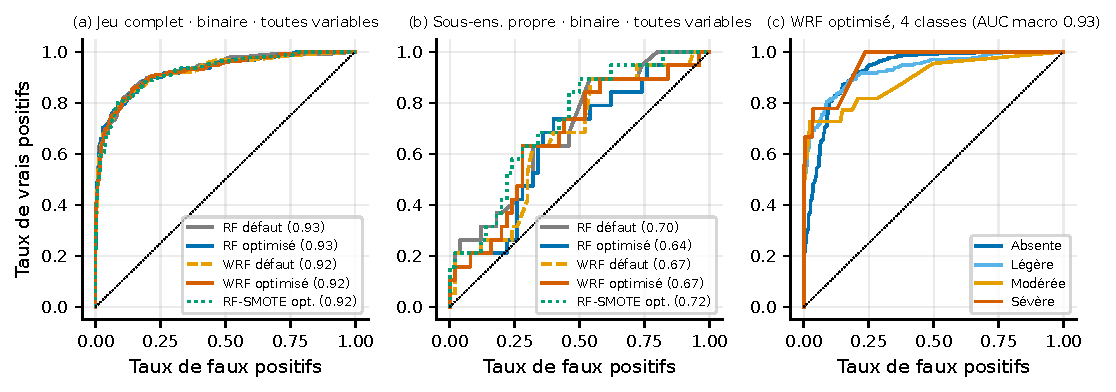
\includegraphics[width=0.92\textwidth]{../figures/roc_curves.pdf}
\caption{Courbes ROC sur le test : binaire, régime complet (a) et propre (b), toutes variables (AUC entre parenthèses) ; WRF optimisée à quatre classes, un-contre-tous (c).}\label{fig:roc}\end{figure*}

\begin{figure*}[t]\centering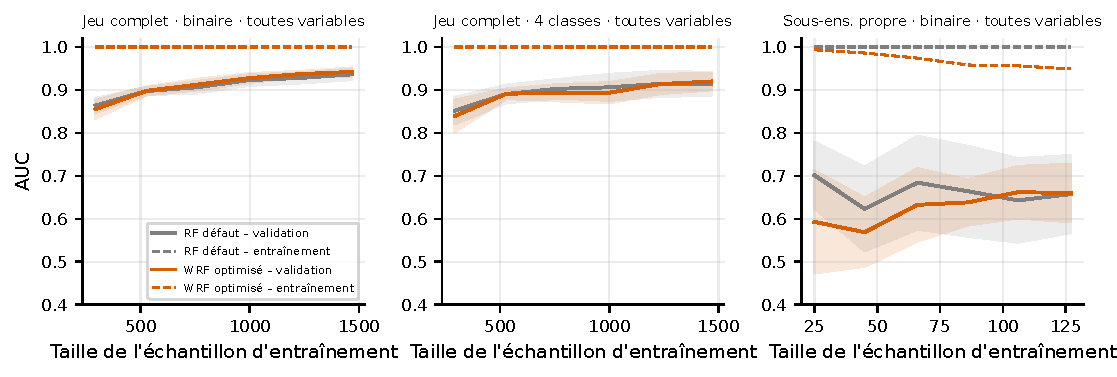
\includegraphics[width=0.92\textwidth]{../figures/learning_curves.pdf}
\caption{Courbes d'apprentissage (validation croisée à 5 plis sur l'entraînement ; bandes : $\pm1$ écart-type).}\label{fig:lc}\end{figure*}

\subsection{Comparaison baseline et améliorations}
\paragraph{Coût de calcul.} Le tableau~\ref{tab:time} met en regard le nombre d'ajustements, le temps et l'AUC en validation croisée. Pour la RF, la recherche aléatoire atteint la même qualité que la grille (0,942 contre 0,941) avec 150 au lieu de 320 ajustements ; Optuna (0,942 pour la WRF, 150 ajustements, 33\,s) fait aussi bien. Pour LR, NB et KNN, le coût est négligeable ; pour l'ANN, 41 à 55\,s de calcul n'apportent aucun gain sur le test dans le régime complet (0,853 $\to$ 0,854 / 0,861). À budget équivalent, aucune des trois stratégies ne domine nettement : le gain tient davantage au \emph{choix du modèle} qu'à celui de la méthode de recherche.

\begin{table}[t]\centering\caption{Coût et score de validation (régime complet, binaire, toutes variables) : nombre d'ajustements, temps réel (s) et AUC en validation croisée.}\label{tab:time}
\scriptsize\begin{tabular}{lcrrrrccc}
\toprule
Modèle & Déf. & \multicolumn{2}{c}{Grid} & \multicolumn{2}{c}{Random} & \multicolumn{3}{c}{AUC-VC} \\\cmidrule(lr){3-4}\cmidrule(lr){5-6}\cmidrule(lr){7-9}
 & (s) & fits & s & fits & s & Déf. & Grid & Rand. \\
\midrule
LR & 0,01 & 50 & 0 & 150 & 1 & 0,762 & 0,762 & 0,762 \\
RF & 0,39 & 320 & 32 & 150 & 25 & 0,935 & 0,941 & 0,942 \\
KNN & 0,01 & 160 & 2 & 150 & 2 & 0,834 & 0,888 & 0,888 \\
SVM & 0,70 & 80 & 9 & 150 & 17 & 0,837 & 0,852 & 0,846 \\
NB & 0,00 & 45 & 0 & 150 & 0 & 0,723 & 0,725 & 0,724 \\
ANN & 1,86 & 160 & 41 & 150 & 55 & 0,883 & 0,883 & 0,883 \\
WLR & 0,01 & 50 & 0 & 150 & 0 & 0,763 & 0,763 & 0,763 \\
WRF & 0,30 & 320 & 31 & 150 & 27 & 0,936 & 0,942 & 0,943 \\
RF-SMOTE & 0,38 & 360 & 45 & 150 & 26 & 0,934 & 0,939 & 0,936 \\
WHGB & 1,29 & 360 & 15 & 150 & 12 & 0,931 & 0,935 & 0,934 \\
\bottomrule
\end{tabular}

\smallskip\noindent\footnotesize Optuna (TPE, WRF) : 150 fits, 33\,s.
\end{table}

\paragraph{Incertitude.} Le tableau~\ref{tab:boot} donne les intervalles de confiance à 95\,\% de l'AUC de test. Dans le régime complet, ils mesurent $\pm 0{,}02$ en binaire et $\pm 0{,}05$ à quatre classes ; dans le régime propre, $\pm 0{,}14$. Pour chaque cadre, les intervalles des quatre variantes se chevauchent ; la plus forte hausse (WRF à quatre classes, toutes variables, $+0{,}024$ sur la WRF par défaut) ne s'en détache donc pas à l'échelle d'un seul découpage, d'où la validation imbriquée ci-dessous.

\begin{table*}[t]\centering\caption{AUC de test et intervalle de confiance \emph{bootstrap} à 95\,\% (1\,000 rééchantillonnages) ; variante optimisée choisie d'après l'AUC en validation croisée.}\label{tab:boot}
\footnotesize\begin{tabular}{lcccc}
\toprule
Cadre & RF défaut & RF optimisé & WRF défaut & WRF optimisé \\
\midrule
Complet, binaire, biomarq. & 0,936 [0,917 ; 0,954] & 0,936 [0,918 ; 0,955] & 0,932 [0,912 ; 0,951] & 0,935 [0,916 ; 0,953] \\
Complet, binaire, toutes var. & 0,928 [0,906 ; 0,948] & 0,926 [0,904 ; 0,946] & 0,923 [0,901 ; 0,945] & 0,925 [0,903 ; 0,945] \\
Complet, 4 classes, biomarq. & 0,898 [0,845 ; 0,951] & 0,893 [0,839 ; 0,949] & 0,896 [0,842 ; 0,947] & 0,896 [0,843 ; 0,950] \\
Complet, 4 classes, toutes var. & 0,895 [0,842 ; 0,943] & 0,895 [0,836 ; 0,946] & 0,903 [0,851 ; 0,950] & 0,927 [0,898 ; 0,954] \\
Propre, binaire, biomarq. & 0,676 [0,530 ; 0,816] & 0,621 [0,477 ; 0,767] & 0,649 [0,503 ; 0,788] & 0,611 [0,464 ; 0,762] \\
Propre, binaire, toutes var. & 0,695 [0,558 ; 0,832] & 0,644 [0,488 ; 0,793] & 0,665 [0,520 ; 0,806] & 0,668 [0,523 ; 0,814] \\
\bottomrule
\end{tabular}
\end{table*}
